\documentclass[mat1, tisk]{fmfdelo}
\usepackage{graphicx}
\usepackage{enumitem}
\usepackage{amsmath}
% \documentclass[fin1, tisk]{fmfdelo}
% Če pobrišete možnost tisk, bodo povezave obarvane,
% na začetku pa ne bo praznih strani po naslovu, …

%%%%%%%%%%%%%%%%%%%%%%%%%%%%%%%%%%%%%%%%%%%%%%%%%%%%%%%%%%%%%%%%%%%%%%%%%%%%%%%
% METAPODATKI
%%%%%%%%%%%%%%%%%%%%%%%%%%%%%%%%%%%%%%%%%%%%%%%%%%%%%%%%%%%%%%%%%%%%%%%%%%%%%%%

% - vaše ime
\avtor{Tadeja Možina}

% - naslov dela v slovenščini
\naslov{Metrična dimenzija grafa deliteljev niča}

% - naslov dela v angleščini
\title{Metric dimension of a zero-divisor graph}

% - ime mentorja/mentorice s polnim nazivom:
%   - doc.~dr.~Ime Priimek
%   - izr.~prof.~dr.~Ime Priimek
%   - prof.~dr.~Ime Priimek
%   za druge variante uporabite ustrezne ukaze
\mentor{izr.~prof.~dr.~David Dolžan}

% - leto diplome
\letnica{2024} 

% - povzetek v slovenščini
%   V povzetku na kratko opišite vsebinske rezultate dela. Sem ne sodi razlaga
%   organizacije dela, torej v katerem razdelku je kaj, pač pa le opis vsebine.
\povzetek{V diplomski nalogi preučujemo metrično dimenzijo grafa deliteljev niča kolobarja.}

% - povzetek v angleščini
\abstract{In this thesis, we study the metric dimension of a zero-divisor graph of a ring.}

% - klasifikacijske oznake, ločene z vejicami
%   Oznake, ki opisujejo področje dela, so dostopne na strani https://www.ams.org/msc/
\klasifikacija{74B05, 65N99}

% - ključne besede, ki nastopajo v delu, ločene s \sep
\kljucnebesede{metrična dimenzija\sep graf deliteljev niča\sep kolobar}

% - angleški prevod ključnih besed
\keywords{metric dimension\sep zero-divisor graph\sep ring} % angleški prevod ključnih besed

% - angleško-slovenski slovar strokovnih izrazov
\slovar{
%\geslo{continuous}{zvezen}
%\geslo{uniformly continuous}{enakomerno zvezen}
%\geslo{compact}{kompakten -- metrični prostor je kompakten, če ima v njem vsako zaporedje stekališče; podmnožica evklidskega prostora je kompaktna natanko tedaj, ko je omejena in zaprta  }
%\geslo{glide reflection}{zrcalni zdrs ali zrcalni pomik -- tip ravninske evklidske izometrije, ki je kompozitum zrcaljenja in translacije vzdolž iste premice}  
%\geslo{lattice}{mreža}  
%\geslo{link}{splet}
%\geslo{partition}{\textbf{$\sim$ of a set} razdelitev množice; \textbf{$\sim$ of a number} razčlenitev števila}
}

% - ime datoteke z viri (vključno s končnico .bib), če uporabljate BibTeX
\literatura{literatura.bib}

%%%%%%%%%%%%%%%%%%%%%%%%%%%%%%%%%%%%%%%%%%%%%%%%%%%%%%%%%%%%%%%%%%%%%%%%%%%%%%%
% DODATNE DEFINICIJE
%%%%%%%%%%%%%%%%%%%%%%%%%%%%%%%%%%%%%%%%%%%%%%%%%%%%%%%%%%%%%%%%%%%%%%%%%%%%%%%

% naložite dodatne pakete, ki jih potrebujete
\usepackage{algpseudocode}  % za psevdokodo
\usepackage{algorithm}      % za algoritme
\floatname{algorithm}{Algoritem}
\renewcommand{\listalgorithmname}{Kazalo algoritmov}

% deklarirajte vse matematične operatorje, da jih bo LaTeX pravilno stavil
% \DeclareMathOperator{\conv}{conv}
% na razpolago so naslednja matematična okolja, ki jih kličemo s parom
% \begin{imeokolja}[morebitni komentar v oklepaju] ... \end{imeokolja}
%
% definicija, opomba, primer, zgled, lema, trditev, izrek, posledica, dokaz

% za številske množice uporabite naslednje simbole
\newcommand{\R}{\mathbb R}
\newcommand{\N}{\mathbb N}
\newcommand{\Z}{\mathbb Z}
% Lahko se zgodi, da je ukaz \C definiral že paket hyperref,
% zato dobite napako: Command \C already defined.
% V tem primeru namesto ukaza \newcommand uporabite \renewcommand
\newcommand{\C}{\mathbb C}
\newcommand{\Q}{\mathbb Q}

%%%%%%%%%%%%%%%%%%%%%%%%%%%%%%%%%%%%%%%%%%%%%%%%%%%%%%%%%%%%%%%%%%%%%%%%%%%%%%%
% ZAČETEK VSEBINE
%%%%%%%%%%%%%%%%%%%%%%%%%%%%%%%%%%%%%%%%%%%%%%%%%%%%%%%%%%%%%%%%%%%%%%%%%%%%%%%

\begin{document}

\section{Uvod}

%Na začetku prvega poglavja/razdelka (ali v samostojnem razdelku z naslovom
%Uvod) napišite kratek zgodovinski in matematični uvod. Pojasnite motivacijo za
%problem, kje nastopa, kje vse je bil obravnavan. Na koncu opišite tudi
%organizacijo dela -- kaj je v kakšnem razdelku.

%Če se uvod naravno nadaljuje v besedilo prvega poglavja, lahko nadaljujete z
%besedilom v istem razdelku, sicer začnete novega. Na začetku vsakega
%razdelka/podraz\-delka poveste, čemu se bomo posvetili v nadaljevanju. Pri
%pisanju uporabljajte ukaze za matematična okolja, med formalnimi enotami
%dodajte vezno razlagalno besedilo.
Pojem metrične dimenzije grafa je v sedemdesetih letih prejšnjega stoletja 
uvedel Peter J. Slater, problem iskanja le te pa sta kot prva raziskovala 
Frank Harary in Robert Melter~\cite{7dolzan}~\cite{4pirzada17}. Uporablja se 
na različnih področjih, kot na primer v farmacevtski kemiji, navigaciji 
robotov in kombinatorični optimizaciji~\cite{0OuSh}.
Formule za metrično dimenzijo poljubnega grafa ni, v diplomski nalogi 
pa bomo navedli različne izreke, ki jo bodo v določenih primerih vseeno 
lahko omejili. Gledali bomo enostavne 
neusmerjene grafe, predvsem pa grafe deliteljev niča poljubnega kolobarja, 
posebej pa bomo pogledali metrični dimenziji grafov deliteljev niča kolobarja 
ostankov po danem modulu in kolobarja matrik nad danim poljem.
%
%
\section{Metrična dimenzija}
V tem poglavju bomo predstavili osnovne pojme, povezane z metrično dimenzijo grafa 
deliteljev niča kolobarja. Pri tem bomo sledili~\cite{0OuSh}. Skozi celotno diplomsko nalogo 
bodo bili vsi grafi neusmerjeni, kolobarji pa bodo vsebovali enico.
%
\subsection{Osnovne definicije}
%
\begin{definicija}
  Naj bo R kolobar in $Z(R)$ njegova množica deliteljev niča.
  \emph{Graf deliteljev niča kolobarja R} je enostaven neusmerjen graf z množico
  vozlišč $Z^{*}(R) = Z(R)\setminus\{0\} $, kjer je med dvema različnima vozliščema $a,b \in Z^{*}(R) $
  povezava natanko tedaj, ko je $ab = 0$ ali $ba = 0$. Označimo ga z $\Gamma(R)$.
\end{definicija}
%
\begin{zgled}\label{prim1}
  Poglejmo si graf deliteljev niča kolobarja $\Z_{10}$. Množica njegovih vozlišč je 
  $V(\Gamma(\Z_{10})) = Z^{*}(\Z_{10}) = \{2, 4, 5, 6, 8\}$, množica povezav pa 
  je enaka $E(\Gamma(\Z_{10})) = \{2 - 5, 4 - 5, 6 - 5, 8 - 5\}$.
  \begin{figure}[H]
    \centering
    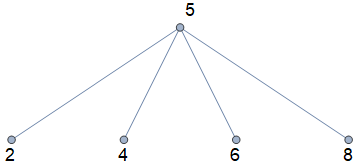
\includegraphics[scale=0.5]{z10.png}
    \caption{Graf deliteljev niča $\Z_{10}$}
  \end{figure}
\end{zgled}
%
\begin{zgled}\label{zgled2.3}
  Poglejmo si še graf deliteljev niča kolobarja $\Z_{12}$. Množica njegovih vozlišč je 
  $V(\Gamma(\Z_{12})) = Z^{*}(\Z_{12}) = \{2, 3, 4, 6, 8, 9, 10\}$, povezave pa so 
  prikazane na sliki.
  \begin{figure}[H]
    \centering
    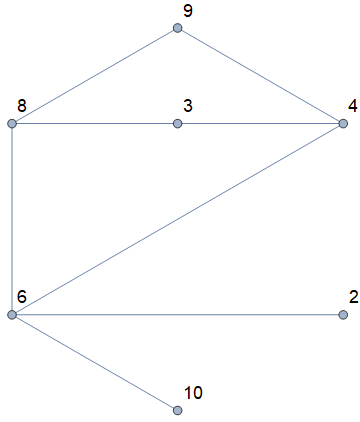
\includegraphics[scale=0.5]{z12.png}
    \caption{Graf deliteljev niča $\Z_{12}$}
  \end{figure}
\end{zgled}
%
Spomnimo se še definicije razdalje med dvema vozliščema v grafu. Za poljubni različni vozlišči 
$u,v \in V(\Gamma)$ je \emph{razdalja} med $u$ in $v$, označena z $d(u,v)$, dolžina 
najkrajše poti med njima. Če ne obstaja pot med $u$ in $v$, je $d(u,v) = \infty $, 
razdalja vozlišča od samega sebe pa je $0$.
Z uporabo razdalje definiramo predstavitev $v$ glede na $W$~\cite{7dolzan}.
%
\begin{definicija}
  Naj bo $W = \{ w_1,w_2, \ldots, w_k \}$ urejena podmnožica množice $V(\Gamma)$ in 
  $v \in V(\Gamma)$. Potem 
  se $k$-dimenzionalni vektor $r(v|W)=( d(v,w_1), \ldots, d(v,w_k) )$ imenuje 
  \emph{predstavitev $v$ glede na $W$}. 

  Rečemo, da je $v$ \emph{rešljiv z W}, če velja $r(v|W) \neq r(u|W)$ 
  za vsak $u \in V(\Gamma)$ različen od $v$, torej 
  $( d(v,w_1), \ldots, d(v,w_k) ) \neq ( d(u,w_1), \ldots, d(u,w_k) )$ za vsak 
  $u \neq v$.
\end{definicija}
%
Množici $W$ pravimo \emph{rešljiva množica grafa $\Gamma$}, če imata poljubni različni 
vozlišči v $V(\Gamma)$ različni predstavitvi glede na $W$. Če je $W$ rešljiva množica 
z najmanjšo močjo, ji pravimo \emph{baza $\Gamma$}.
%
%Metrična dimenzija
\begin{definicija}
  \emph{Metrična dimenzija grafa $\Gamma$} je moč njegove baze. Označimo jo z $dim(\Gamma)$.
\end{definicija}
%
\begin{opomba}\label{opomba2.7}
  %dovolj je gledati predstavitve elementov izven W glede na W.
  Če preverjamo, ali je $W= \{w_1,w_2, \ldots, w_k\} \subseteq V(\Gamma)$ 
  rešljiva množica $\Gamma$, je dovolj gledati predstavitve elementov iz 
  $V(\Gamma) \setminus W$ glede na $W$. Namreč če izberemo $w_i \in W$ bo vektor 
  $(d(w_i,w_1),d(w_i,w_2), \ldots d(w_i,w_k))$ na $i$-tem mestu imel 0. 
  Če bi katerokoli drugo vozlišče $u$ imelo enako predstavitev kot $w_i$, bi 
  potem moralo veljati, da $d(w_i,w_i) = d(u,w_i)$, kar pa je edino možno, 
  če je $u = w_i$.
\end{opomba}
%
\begin{opomba}\label{opomba2.8}
  Očitno je vsaka nadmnožica rešljive množice grafa $\Gamma$ tudi sama rešljiva 
  množica. Res, naj bo $W_2$ nadmnožica rešljive množice $W_1$ grafa $\Gamma$, 
  torej $W_1 \subseteq W_2$. Po opombi \ref{opomba2.7} je dovolj gledati 
  predstavitve elementov izven $W_2$. Ker so predstavitve teh elementov glede na 
  $W_1$ različne in $W_2$ vsebuje $W_1$, bodo njihove predstavitve glede na 
  $W_2$ bile enake tistim v $W_1$ z nekaj dodanimi komponentami, torej še vedno 
  različne.
\end{opomba}
%
\begin{zgled}\label{prim1.2}
  Poiščimo metrično dimenzijo grafa deliteljev niča kolobarja $\Z_{10}$ iz 
  primera \ref{prim1}. Razdalje 
  med dvema poljubnima različnima vozliščema so 1 ali 2. Če za $W = \{w\}$ vzamemo 
  katerokoli enoelementno množico, bosta obstajali vsaj dve vozlišči iz 
  $\{2,4,6,8\}$, ki imata enako razdaljo do $w$, torej to ni baza. Podoben razmislek 
  naredimo, če je $W$ dvoelementna množica - v $\{2,4,6,8\}$ bosta obstajali dve 
  vozlišči z enako predstavitvijo glede na $W$. Poglejmo sedaj, če obstaja rešljiva 
  množica moči 3. Vzemimo $W = \{2,4,6\}$. Edina dva elementa, ki ju rabimo pogledati 
  sta 5 in 8. Izračunamo 
  $(d(5,2),d(5,4),d(5,6)) = (1,1,1) \neq (d(8,2),d(8,4),d(8,6)) = (2,2,2)$. Torej je 
  metrična dimenzija $\Gamma(\Z_{10})$ = 3.
\end{zgled}
%
\begin{opomba}
  Graf $\Gamma$ ima lahko več rešljivih množic iste moči. Pri zgledu \ref{prim1.2} 
  bi za rešljivo množico moči 3 (in torej tudi bazo) tako lahko vzeli tudi 
  $\{2,4,8\}$, $\{2,6,8\}$ ali $\{4,6,8\}$.
\end{opomba}
%
\subsection{Meje metrične dimenzije grafa}
%
Ponovimo nekaj pojmov, ki jih bomo potrebovali v nadaljevanju. Za končen graf 
$\Gamma = (V, E)$ je njegov \emph{premer}, označen z $diam(\Gamma)$, največja 
razdalja med dvema vozliščema v grafu. \emph{Soseščina} vozlišča $v$ je 
množica $N(v) = \{ x \in V(\Gamma)~|~x \sim v \}$, torej množica vozlišč 
s katerimi ima $v$ povezavo. 

Navedimo sedaj prvo trditev, ki postavi meje metrične dimenzije grafa~\cite{10chartrand}.
%
\begin{trditev}
  Naj bo $\Gamma$ povezan graf z $n$ vozlišči in premerom $d$ = $diam(\Gamma)$. Potem velja
  $n - d^{dim(\Gamma)} \leq dim(\Gamma) \leq n - d$.
\end{trditev}
\begin{dokaz}
  Poglejmo si najprej drugo neenakost. Naj bosta $u$ in $v$ vozlišči grafa 
  $\Gamma$, pri katerih je razdalja največja možna, torej $d(u,v) = d$. 
  Njuno $uv$-pot dolžine $d$ zapišemo kot $u=v_0, v_1, \ldots, v_d=v$. 
  Naj bo $W = V(\Gamma) \setminus \{v_1, \ldots, v_d \}$. Potem je 
  $d(u,v_i) = i$ za $i = 1, \ldots, d$. Ker je $u \in W$ in imajo 
  vsa vozlišča grafa izven $W$ paroma različno razdaljo do $u$ in 
  torej različno predstavitev glede na $W$, je $W$ 
  rešljiva množica $\Gamma$.

  Za dokaz prve neenakosti izberimo bazo $B$ grafa $\Gamma$ moči $k$. 
  Poglejmo vozlišča iz $V(\Gamma) \setminus B$, teh je $n-k$. 
  Njihove predstavitve 
  glede na $B$ so vektorji dolžine $k$, katerih komponente so števila med 
  $1$ in $d$. Vsakemu vozlišču iz $V(\Gamma) \setminus B$ priredimo 
  tak vektor. Ker je $B$ baza, morajo biti vektorji med sabo različni. 
  Torej je preslikava injektivna in dobimo $n - k \leq d^k$. 
  Neenakost preuredimo in dobimo željen rezultat.
\end{dokaz}
%
Navedimo še nekaj novih definicij, s katerimi si bomo pomagali še dodatno 
izboljšati meje metrične dimenzije grafa.
%
\begin{definicija}
  Za različni vozlišči $u, v\in V(\Gamma)$ pravimo, da sta \emph{dvojčka}, če velja 
  $N(u) \cup \{u\} = N(v) \cup \{v\} $, ko $u \sim v$, ali 
  $N(u) = N(v) $, ko $u \nsim v$.

  Množico dvojčkov vozlišča $v$ označimo s $Tw(v)$.
\end{definicija}
%
Opazimo, da $V(\Gamma)$ lahko zapišemo kot disjunktno unijo množic 
dvojčkov, saj vsaka množica dvojčkov $Tw(v)$ vsebuje vsaj en element, vozlišče $v$, 
poleg tega pa je vsako vozlišče v natanko eni taki množici.
Glede na to, koliko vozlišč vsebujejo, množice dvojčkov delimo v dve skupini.
%
\begin{definicija}
  Množici dvojčkov $Tw(v)$ pravimo, da je \emph{prava množica dvojčkov grafa $\Gamma$}, 
  če je $|Tw(v)| \geq 2$. Če je $|Tw(v)| = 1$, ji rečemo 
  \emph{osamljena množica dvojčkov grafa $\Gamma$}. 

  Število pravih množic dvojčkov grafa $\Gamma$ označimo z \emph{$\alpha(\Gamma)$}, število 
  osamljenih množic dvojčkov pa z \emph{$\beta(\Gamma)$}.
\end{definicija}
%
\begin{zgled}
  Poglejmo množice dvojčkov iz zgleda \ref{zgled2.3}. Te so 
  $\{9,3\},$ $\{8,4\},\{2,10\}$ in $\{6\}$. Število pravih množic dvojčkov grafa $\Gamma(\Z_{12})$ 
  je torej $\alpha(\Gamma(\Z_{12})) = 3$, število osamljenih pa $\beta(\Gamma(\Z_{12})) = 1$.
\end{zgled}
%
Navedimo sedaj trditev, ki uporabi množice dvojčkov za omejitev metrične 
dimenzije grafa~\cite{3pirzada14}.
%
\begin{trditev}\label{trditev2.14}
  Naj bo $\Gamma$ povezan graf in $T_1, T_2, \ldots, T_{\alpha(\Gamma)}$ različne 
  prave množice dvojčkov grafa $\Gamma$. Potem velja:
  \begin{enumerate}[label=(\roman*)]
    \item Vsaka rešljiva množica grafa $\Gamma$ vsebuje vsa, razen morda enega, vozlišča iz 
          vsakega $T_i$, za $1 \leq i \leq \alpha(\Gamma)$,
    \item Obstaja baza $B$ grafa $\Gamma$, da $B$ vsebuje največ $|T_i| - 1$ vozlišč 
          iz vsakega $T_i$, za $1 \leq i \leq \alpha(\Gamma)$,
    \item $|V(\Gamma)| - \alpha(\Gamma) - \beta(\Gamma) \leq dim(\Gamma) \leq |V(\Gamma)| - \alpha(\Gamma)$.
  \end{enumerate}
\end{trditev}
\begin{dokaz}
  Dokažimo najprej točko i). Naj bo $W$ baza $\Gamma$. Recimo, da trditev ne velja, 
  torej da obstajata vozlišči $u,v$ v isti pravi množici dvojčkov, ki obadva nista v $W$. 
  Naj bo ta množica dvojčkov $T_i$. Ker sta $u$ in $v$ v isti množici dvojčkov, 
  imata enake sosede, torej je njuna predstavitev glede na $W$ enaka, kar pa ni 
  možno, saj je $W$ rešljiva množica.

  Dokažimo sedaj točko ii). Naj bo $B$ rešljiva množica $\Gamma$ in 
  $T_1, T_2, \ldots, T_{\alpha(\Gamma)}$ njene prave množice dvojčkov ter 
  $T_{\alpha(\Gamma)+1}, \ldots, T_{\alpha(\Gamma)+\beta(\Gamma)}$ osamljene množice dvojčkov.
  Brez škode za splošnost naj bo $\alpha(\Gamma) > 0$, torej $|T_1| > 1$. 
  Naj bo $W$ rešljiva množica grafa, ki vsebuje $T_1$, in naj bo $x \in T_1$. 
  Ker je $x \in W$, je množica $W$ je oblike $W = \{x, w_1, w_2, \ldots\}$.
  Pokazali bomo, da če je $W$ rešljiva množica grafa $\Gamma$, ki vsebuje $T_1$, lahko 
  množici $W$ odstranimo en element $x \in T_1$, da je ali $P_1 = W \setminus \{x\}$ 
  rešljiva množica ali pa obstaja osamljena množica dvojčkov $\{s\}$, da je 
  $P_2 = (W \cup \{s\}) \setminus \{x\}$ rešljiva množica. Tako skonstruirana rešljiva 
  množica bo imela moč manjšo ali enako $W$ in bo vsebovala vse, razen enega, vozlišča 
  iz prave množice dvojčkov $T_1$. Postopek potem ponovimo še za ostale prave množice dvojčkov 
  in končna rešljiva množica bo vsebovala največ $|T_i| - 1$ vozlišč 
  iz vsakega $T_i$, za $1 \leq i \leq \alpha(\Gamma)$.

  Definirajmo množico $P_1 = W \setminus \{x\} = \{w_1, w_2, \ldots\}$ in poglejmo, kdaj je 
  rešljiva. Po opombi \ref{opomba2.7} je dovolj preverjati, da so predstavitve elementov 
  izven $P_1$ glede na $P_1$ različne. Poglejmo najprej za $u_1, u_2 \notin W$. Recimo, da je 
  $r(u_1|P_1) = r(u_2|P_1)$. Ker je $W$ rešljiva množica, že vemo, da se njuni predstavitvi 
  glede na $W$ razlikujeta, $r(u_1|W) \neq r(u_2|W)$. Iz tega sledi, da imata $u_1$in $u_2$ 
  različno razdaljo do $x$-a, torej $d(u_1, x) \neq d(u_2, x)$. Vemo tudi, da ker velja 
  $|T_1| > 1$ in $T_1 \subseteq W$, obstaja $z \in T_1 \cap P_1$, $z \neq x$. Ker je $z \in P_1$, 
  iz $r(u_1|P_1) = r(u_2|P_1)$ sledi, da $d(u_1, z) = d(u_2, z)$. Po drugi strani, pa 
  sta $x$ in $z$ v isti množici dvojčkov, torej so njune razdalje do elementov enake. 
  Dobimo $d(u_1, x) = d(u_1, z) = d(u_2, z) = d(u_2, x)$, kar pa nas pripelje v 
  protislovje. Torej, če za $u_1, u_2 \notin P_1$ velja $r(u_1|P_1) = r(u_2|P_1)$, 
  mora biti eden izmed njiju enak $x$. Če ne obstaja tak $u_1 \notin P_1$, $u_1 \neq x$, da 
  velja $r(u_1|P_1) = r(x|P_1)$, potem je $P_1$ rešljiva množica. V nasprotnem primeru 
  pokažimo, da obstaja $s \in V(\Gamma) \setminus T_1$,
  da je $P_2 = (W \cup \{s\}) \setminus \{x\}$ rešljiva množica.

  Recimo sedaj, da obstaja tak $u_1 \notin P_1$, da $r(u_1|P_1) = r(x|P_1)$. Pokažimo, da je 
  tak $u_1$ en sam. Recimo, da obstaja še en $u_2 \notin P_1$, da 
  $r(u_2|P_1) = r(u_1|P_1) = r(x|P_1)$. Naj bo $z \in T_1 \cap P_1$, $z \neq x$. Podobno kot prej, iz 
  dejstva, da je $W$ rešljiva množica, sledi, da je $d(u_2, x) \neq d(u_1, x)$. Ker pa je 
  $r(u_2|P_1) = r(u_1|P_1)$ in sta $z$ in $x$ v isti množici dvojčkov, dobimo 
  $d(u_1, x) = d(u_1, z) = d(u_2, z) = d(u_2, x)$, s čimer pridemo v protislovje. Torej je 
  tak $u_1$ en sam. Sedaj razdelimo možnosti glede na to, koliko je $\beta(\Gamma)$.

  Naj bo $\beta(\Gamma) = 0$, torej $|T_i| \geq 2$ za vsak $i = 1, \ldots, k$. Poglejmo 
  poljuben $y \in V(\Gamma) \setminus \{x, u_1\}$. Ker so vse množice dvojčkov prave in 
  po točki i) rešljiva množica $W$ vsebuje vsa, razen mogoče enega, vozlišča in vsakega $T_i$, 
  obstaja $q \in P_1$, ki je v isti množici dvojčkov kot $y$. Dobimo enakost 
  $d(u_1, y) = d(u_1, q) = d(x, q) = d(x, y)$. Ker je bil $y$ poljuben, sledi, da 
  sta $x$ in $u_1$ v isti množici dvojčkov, kar pa nas pripelje v protislovje s 
  tem, da je $x$ edini element množice dvojčkov $T_1$, ki ni v $W$.

  Naj bo sedaj $\beta(\Gamma) > 0$. Brez škode za splošnost naj bo $|T_j| = 1$ za neki $j \neq 1$. 
  Ker $u_1$ in $x$ nista v isti množici dvojčkov, 
  obstaja $s \in V(\Gamma) \setminus \{x, u_1\}$, da $d(x, s) \neq d(u_1, s)$. Če je $s \in P_1$, 
  dobimo protislovje s $r(u_1|P_1) = r(x|P_1)$, torej je $s \notin P_1$. Dokažimo sedaj, 
  da je tak $s$ tudi v osamljeni množici dvojčkov. Označimo s $T_l$ množico dvojčkov, v kateri 
  je $s$, in recimo, da je v njej še eno drugo vozlišče $l \in T_l$. Po točki i) rešljiva 
  množica $W$ vsebuje vse razen mogoče enega vozlišča, torej je $l$ v $P_1$. 
  Iz tega in iz $r(u_1|P_1) = r(x|P_1)$ dobimo enakost 
  $d(u_1, s) = d(u_1, l) = d(x, l) = d(x, s)$, kar pa je v 
  protislovju s $d(x, s) \neq d(u_1, s)$. Torej je $T_l = \{s\}$. Poglejmo sedaj 
  $P_2 = P_1 \cup \{s\} = (W \cup \{s\}) \setminus \{x\}$. Očitno je $|P_2| = |W|$. Opazimo, 
  da iz $d(x, s) \neq d(u_1, s)$ sledi, da je $r(x|P_2) \neq r(u_1|P_2)$. Dokažimo še, da je 
  $P_2$ rešljiva množica. Recimo, da ni, torej, da obstajata $a, b \notin P_2$, ki imata 
  enaki predstavitvi glede na $P_2$. Ker je $P_1 \subseteq P_2$ sledi, 
  da $a, b \notin P_1$. Podobno kot prej lahko pokažemo, da če velja $r(a|P_2) = r(b|P_2)$, 
  potem mora eden izmed njiju biti $x$, brez škode za splošnost naj bo to $a$. Po že prej 
  dokazanem pa če tak $b$ obstaja, da je $r(x|P_2) = r(b|P_2)$, je enolično določen, 
  torej $b = u_1$. Vendar $u_1 = b$ in $x = a$ imata različno predstavitev glede na $s \in P_2$, 
  torej $r(a|P_2) \neq r(b|P_2)$ in dobimo protislovje. Torej je $P_2$ rešljiva množica.

  Nazadnje dokažimo še točko iii). Po točki ii) obstaja baza $P$, ki ima iz vsake 
  množice dvojčkov $T_i$, $1 \leq i \leq \alpha(\Gamma)$ največ $|T_i| - 1$ vozlišč. 
  Torej $P$ je baza, ki ima največ $|V(\Gamma)| - \alpha(\Gamma)$ vozlišč in 
  posledično je $dim(\Gamma) \leq |V(\Gamma)| - \alpha(\Gamma)$. Spodnjo mejo dokažimo s 
  pomočjo točke i). Naj bodo $T_1, \ldots, T_{\alpha(\Gamma)}$ prave množice dvojčkov ter 
  $T_{\alpha(\Gamma)+1}, \ldots, T_{\alpha(\Gamma)+\beta(\Gamma)}$ osamljene množice dvojčkov. 
  Po točki i) vsaka rešljiva množica vsebuje vse, razen morda enega, vozlišča iz 
  $T_1, \ldots, T_{\alpha(\Gamma)}$. Če upoštevamo, da je osamljenih množic $\beta(\Gamma)$, 
  dobimo $|V(\Gamma)| - \alpha(\Gamma) - \beta(\Gamma) \leq dim(\Gamma)$.
\end{dokaz}
%
Navedimo še lemo, ki nam pove, kdaj je metrična dimenzija grafa spodnja meja iz 
točke (iii) trditve \ref{trditev2.14}~\cite{0OuSh}.
%
\begin{lema}\label{lema2.15}
  Naj bo $\Gamma$ povezan graf. Če vsako vozlišče iz osamljenih množic dvojčkov 
  grafa $\Gamma$ ni vsebovano v nobeni bazi grafa $\Gamma$, potem je 
  $dim(\Gamma) = |V(\Gamma)| - \alpha(\Gamma) - \beta(\Gamma)$.
\end{lema}
\begin{dokaz}
  Naj bo $\Gamma$ povezan graf, $T_1, \ldots, T_{\alpha(\Gamma)}$ njegove prave množice dvojčkov in 
  $T_{\alpha(\Gamma)+1}, \ldots, T_{\alpha(\Gamma)+\beta(\Gamma)}$ njegove osamljene množice 
  dvojčkov. Po točki (ii) trditve \ref{trditev2.14} obstaja 
  baza $B$ grafa $\Gamma$, ki vsebuje največ $|T_i| - 1$ vozlišč 
  iz vsake prave množice dvojčkov $T_i$. Torej $|B \cap T_i| \leq |T_i| - 1$ 
  za $1 \leq i \leq \alpha(\Gamma)$. Po predpostavki je $|B \cap T_j| = \emptyset$ 
  za $\alpha(\Gamma) + 1 \leq j \leq \alpha(\Gamma) + \beta(\Gamma)$, torej je 
  $dim(\Gamma) = \sum\limits_{i=1}^{\alpha(\Gamma)} |B \cap T_i| \leq 
  \sum\limits_{i=1}^{\alpha(\Gamma)} (|T_i| - 1) = |V(\Gamma)| - \alpha(\Gamma) - \beta(\Gamma)$. 
  Po točki (iii) trditve pa velja $|V(\Gamma)| - \alpha(\Gamma) - \beta(\Gamma) \leq dim(\Gamma)$, 
  torej velja enakost.
\end{dokaz}
%
%
%
\section{Kolobar ostankov}
V tem razdelku si bomo ogledali metrično dimenzijo kolobarja ostankov po danem modulu. 
Pri tem bomo sledili~\cite{3pirzada14}. Metrično dimenzijo $\Gamma(\Z_{n})$ poiščemo 
s pomočjo praštevilskega razcepa $n$. Če je $n$ praštevilo, je graf deliteljev 
niča od $\Z_{n}$ prazen graf, na tem pa metrična dimenzija ni definirana. Poglejmo sedaj 
koliko je metrična dimenzija $\Gamma(\Z_{n})$, če je $n$ produkt dveh različnih praštevil. 
Zato pa najprej navedimo lemo.
%
\begin{lema}\label{lema3.1}
  Naj bo $R$ komutativen kolobar.
  \begin{enumerate}[label=({\alph*})]
    \item Če je $\Gamma(R)$ poln dvodelen graf, različen od $K_{1,1}$, je $dim(\Gamma(R)) = |Z^*(R)| - 2$,
    \item Če je $\Gamma(R)$ poln graf, je $dim(\Gamma(R)) = |Z^*(R)| - 1$.
    \end{enumerate}
\end{lema}
\begin{dokaz}
  Dokažimo naprej točko a).
  Naj bo $\Gamma(R)$ poln dvodelen graf in $U$ in $V$ disjunktni množici vozlišč, da velja, da je 
  vsako vozlišče v $U$ povezano z vsakim vozliščem v $V$ in obratno. 
  Brez škode za splošnost naj bo $|U| \leq |V|$. Ločimo primera glede na moč množice $U$.

  Če je $|U| = 1$ in $|V| = n \geq 2$, dobimo zvezdast graf $K_{1,n}$. Označimo $U = \{u\}$, vozlišča množice 
  $V$ pa z $\{v_1, \ldots, v_n\}$. Očitno je $U$ osamljena množica dvojčkov, $V$ pa prava množica dvojčkov, 
  saj imajo vsa vozlišča v $V$ samo enega soseda, vozlišče $u$. Po točki (iii) trditve \ref{trditev2.14} tako 
  dobimo oceno $|Z^*(R)| - 2 \leq dim(\Gamma(R)) \leq |Z^*(R)| - 1$. Dokažimo sedaj, da že spodnja meja   
  zadošča. Vzemimo $W = \{v_1, v_2, \ldots, v_{n-1}\}$. Predstavitev $u$ glede na $W$ je 
  $r(u|W)=( 1, 1, \ldots, 1 )$, predstavitev $v_n$ glede na $W$ pa $r(v_n|W)=( 2, 2, \ldots, 2 )$. 
  Predstavitvi glede na $W$ sta različni, torej 
  je $W$ res rešljiva množica moči $|Z^*(R)| - 2$.

  Če je $|U| \geq 2$, sta očitno $U$ in $V$ dve različni pravi množici dvojčkov, osamljenih množic dvojčkov 
  pa ta graf nima. Ponovno uporabimo trditev \ref{trditev2.14} in dobimo oceno 
  $|Z^*(R)| - 2 \leq dim(\Gamma(R)) \leq |Z^*(R)| - 2$.

  Dokažimo še točko b). Če je $\Gamma(R)$ poln graf z vsaj dvema vozliščema, imamo samo eno pravo 
  množico dvojčkov (vsa vozlišča grafa), 
  osamljenih množic dvojčkov pa ni. Po točki (iii) trditve \ref{trditev2.14} dobimo oceno 
  $|Z^*(R)| - 1 - 0 \leq dim(\Gamma(R)) \leq |Z^*(R)| - 1$, torej je $dim(\Gamma(R)) = |Z^*(R)| - 1$.
  
  Poglejmo še primer, ko je $\Gamma(R)$ poln graf s samo enim vozliščem. Rešljiva množica 
  je že prazna množica $\{\}$, saj imata poljubni različni vozlišči
  različni predstavitvi glede na prazno množico. Očitno je to rešljiva množica z najmanjšo močjo, torej je 
  $dim(\Gamma(\Z_{4})) = 0$.
\end{dokaz}
%
\begin{trditev}
  Naj bo $n$ produkt dveh različnih praštevil, $n = p \cdot q$. Potem je 
  $dim(\Gamma(\Z_{n})) = p + q - 4$.
\end{trditev}
\begin{dokaz}
  Vemo že, da če sta $p$ in $q$ različni praštevili, lahko $\Z_{n}$ zapišemo kot 
  $\Z_{n} \cong \Z_{p} \times \Z_{q}$. Vozlišča grafa $\Gamma(\Z_{p} \times \Z_{q})$ so 
  torej oblike $ \{(a,b)~|~a \in \Z_{p}, b \in \Z_{q}\}$, kjer sta dve vozlišči $(a_1, b_1)$ in 
  $(a_2, b_2)$ povezani natanko tedaj, ko je $a_1 \cdot a_2 \equiv 0~(mod~p)$ in $b_1 \cdot b_2 \equiv 0~(mod~q)$. 
  Ker pa sta $p$ in $q$ praštevili, je pa to natanko tedaj ko je eden izmed $a_i$ enak $0$ za $i = 1,2$ 
  in eden izmed $b_i$ enak $0$ za $i = 1,2$. Označimo $V_1 =\{ (a,0)~|~a \in \Z_{p}^*\}$ in 
  $V_2 =\{ (0,b)~|~b \in \Z_{q}^*\}$. Vozlišča grafa $\Gamma(\Z_{p} \times \Z_{q})$ so torej 
  elementi množice $V_1 \cup V_2$, vsa 
  vozlišča v $V_1$ pa so povezana z vsemi vozlišči v $V_2$ in obratno. 
  Torej je $\Gamma(\Z_{p} \times \Z_{q})$ poln dvodelen graf $K_{p-1, q-1}$. Uporabimo točko a)
  leme \ref{lema3.1} in dobimo $dim(\Gamma(\Z_{n})) = dim(\Gamma(\Z_{p} \times \Z_{q})) = (p - 1) + (q - 1) - 2 = p + q - 4$.
\end{dokaz}
%
Spomnimo se sedaj še definicije karakteristike in navedimo lemo, ki nam bo pomagala dokazati 
naslednjo trditev~\cite{PIRZADA2019}. \emph{Karakteristika} kolobarja $R$ je najmanjše naravno število $n$, da je 
$n \cdot 1 = 0$. Če tak $n$ ne obstaja, rečemo, da je karakteristika $R$ enaka $0$.
%
\begin{lema}\label{lema3.3}
  Naj bo $R$ končen komutativen kolobar z liho karakteristiko, ki vsebuje neničelne delitelje niča. Naj 
  ima $\Gamma(R)$ natanko $k$ množic dvojčkov. Potem je $dim(\Gamma(R)) = |Z^*(R)| - k$.
\end{lema}
\begin{dokaz}
  Naj bo $x \in Z^*(R)$. Naj bo $N(x)$ soseščina $x$-a in $Tw(x)$ njegova množica dvojčkov. Hitro lahko 
  preverimo, da je sta $x$ in $-x$ v isti množici dvojčkov. Naj bo $y \in N(x)$ poljuben, torej naj zanj 
  velja $x \cdot y = 0$. Računamo $-x \cdot y = - (x \cdot y)= 0$, torej $-x \in Tw(x)$. Obratno, naj 
  bo $z \in N(x)$. Enakost $-x \cdot z = 0$ z leve množimo z $-1$ in dobimo $x \in Tw(-x)$. Torej 
  $Tw(x) = Tw(-x)$. Dokažimo sedaj, da $x \neq -x$. Recimo, da to ni res. Potem velja $0 = x + (-x) = x + x = 2x$. 
  Iz definicije karakteristike sledi, da karakteristika deli $2x$. Po predpostavki pa je liha, torej 
  sta si $2$ in karakteristika kolobarja $R$ tuji naravni števili. Vemo že, da potem obstajata taki 
  celi števili $m$ in $n$, da velja $1 = m \cdot 2 + n \cdot kar(R)$. Enačbo množimo z $x$ in 
  dobimo $x = 1 \cdot x = m \cdot 2 \cdot x + n \cdot kar(R) \cdot x = 0$, torej je $x = 0$, 
  kar pa je v protislovju z 
  neničelnostjo $x$-a. Vse množice dvojčkov so torej prave množice dvojčkov, saj vsebujejo dve različni 
  vozlišči $x$ in $-x$. Uporabimo točko iii) trditve \ref{trditev2.14} in dobimo $dim(\Gamma(R)) = |Z^*(R)| - k$.
\end{dokaz}
%
\begin{trditev}
  Naj bo $p$ praštevilo.
  \begin{enumerate}[label=(\roman*)]
      \item Če je $n = p^2$ in $p \geq 2$, potem je $dim(\Gamma(\Z_{n})) = p - 2$,
      \item Če je $n = p^k$ in $k \geq 3$, potem je $dim(\Gamma(\Z_{n})) = p^{k-1} - k$.
  \end{enumerate}
\end{trditev}
\begin{dokaz}
  Dokažimo najprej točko (i).
  Poglejmo, kaj so vozlišča grafa $\Gamma(\Z_{n})$, kjer je $n = p^2$ in $p > 2$. Dve 
  različni vozlišči $a, b \in \Z_{p^2}$ sta povezani natanko tedaj, ko je njun produkt enak $0$ po modulu 
  $p^2$. Ker pa sta $a$ in $b$ neničelni, je pa to natanko tedaj, ko ima vsak izmed njiju v svojem praštevilskem 
  razcepu natanko en $p$. Vozlišča grafa so torej večkratniki števila $p$, torej množica $\{p,2p,  \ldots, (p-1)p\}$.
  Očitno so vsa vozlišča med seboj povezana in dobimo poln graf na $p-1$ vozliščih. Uporabimo točko b)
  leme \ref{lema3.1} in dobimo $dim(\Gamma(\Z_{p^2})) = p - 1 - 1 = p - 2$.

  Dokažimo sedaj še točko (ii). 
  %
  %Če $p \neq 2$ in $k \geq 3$, podobno kot pri točki (i) vidimo, da so vozlišča grafa 
  %$\Gamma(\Z_{p^k})$ spet večkratniki $p$, torej $V(\Gamma(\Z_{p^k})) = \{p,2p, 3p, \ldots, (p^{k-1}-1)p\}$ 
  %ter da sta dve vozlišči povezani takrat, ko se vsota potenc števila $p$ v njunih praštevilskih 
  %razcepih sešteje v $k$. 
  Podobno kot pri točki (i) vidimo, da so vozlišča grafa 
  $\Gamma(\Z_{p^k})$ spet večkratniki $p$, torej $V(\Gamma(\Z_{p^k})) = \{p,2p, 3p, \ldots, (p^{k-1}-1)p\}$.
  Vsako vozlišče $a$ lahko zapišemo v obliki $a = u p^{k_1}$, kjer je $k_1$ največja možna potenca 
  števila $p$ v množici $\{1, 2, \ldots, k-1\}$, $u$ pa obrnljiv element v $\Z_{p^k}$. Zakaj je $u$ obrnljiv 
  element? Neobrnljivi elementi v $\Z_{p^k}$ so natanko večkratniki $p$, torej če $u$ ne bi bil obrnljiv, bi 
  lahko zapisu števila $a$ dodali še en $p$, kar pa je v protislovju s tem, da je $k_1$ največja možna potenca. 
  Podobno kot pri točki (i), sta dve različni vozlišči $a = u_1 p^{k_1}$ in $b = u_2 p^{k_2}$ povezani takrat, ko je 
  $k_1 + k_2 \geq k$, vozlišče $a$ pa je povezano natanko z vsemi vozlišči pri katerih je potenca pri $p$ 
  večja ali enaka $k - k_1$. 
  Množice dvojčkov so torej oblike $V_i = \{u p^i~|~  u \in  \Z_{p^k}^{*}\}$, kjer $i \in \{1, 2, \ldots, k-1\}$. 
  Sedaj ločimo primera glede na to, ali je $p$ enak $2$ ali ne.

  Če je $p \neq 2$, potem je karakteristika $\Z_{p^k}$ liha. Uporabimo lemo \ref{lema3.3} in dobimo 
  $dim(\Gamma(\Z_{p^k})) = |Z^*(\Z_{p^k})| - (k - 1) = (p^{k-1} - 1) - (k - 1) = p^{k-1} - k$.

  Naj bo sedaj $p = 2$. Poglejmo množice dvojčkov $V_i = \{u 2^i~|~  u \in  \Z_{2^k}^{*}\}$, kjer 
  $i \in \{1, 2, \ldots, k-1\}$. Za $i \in \{1, 2, \ldots, k-2\}$ bodo bile $V_i$ prave množice dvojčkov, saj 
  bodo poleg $2^i$ vsebovale še $-2^i$. Res, če bi veljalo $-2^i = 2^i$, bi lahko na obeh straneh prišteli 
  $2^i$ in dobili $0 = 2 \cdot 2^i = 2^{i+1}$, kar pa nas pripelje v protislovje, saj je karakteristika 
  kolobarja $\Z_{2^k}$ enaka $2^k$, kar pa je večje od $2^{i+1}$ za $i \in \{1, 2, \ldots, k-2\}$.
  Za $i = k-1$ pa preverimo, da je $V_{k-1}$ osamljena množica dvojčkov. Naj bo $u \in \Z_{2^{k-1}}^{*}$. 
  Očitno so obrnljivi elementi v $\Z_{2^{k}}$ liha števila, torej je $u$ oblike $u = 2m + 1$ za nek 
  $m \in \N$. Potem je $u \cdot 2^{k-1} = (2m + 1) \cdot 2^{k-1} = m \cdot 2^{k} + 2^{k-1} \equiv 2^{k-1} ~(mod~2^{k})$. 
  Torej je $u \cdot 2^{k-1} = 2^{k-1}$ za vsak $u \in \Z_{2^{k}}^{*}$ in $V_{k-1}$ je osamljena 
  množica dvojčkov. Po točki i) 
  trditve \ref{trditev2.14} vsaka rešljiva množica, in torej tudi baza, grafa $\Gamma(\Z_{2^k})$ 
  vsebuje vsa, razen morda enega, vozlišča iz vsake prave množice dvojčkov. Naj bo 
  $B$ poljubna baza. Poglejmo, ali je vozlišče $2^{k-1}$ tudi v $B$. Očitno je edino vozlišče povezano z 
  vsemi ostalimi vozlišči v grafu, torej s predstavitvijo glede na $B$ enako 
  $r(2^{k-1}|B) = (1, \ldots, 1)$. Iz tega sledi, da $2^{k-1} \notin B$. Torej je 
  $dim(\Gamma(\Z_{2^{k}})) = |Z^*(\Z_{2^k})| - (k - 2) - 1 = (2^{k-1} - 1) - (k - 1) = 2^{k-1} - k$.
\end{dokaz}
%
Ponovimo sedaj definicijo Eulerjeve funkcije $\varphi(n)$~\cite{wiki:xxx}. \emph{Eulerjeva funkcija $\varphi (n)$} 
je funkcija naravnega števila $n$, ki nam pove, koliko je naravnih števil manjših od $n$, ki so z $n$ tuja. 
S pomočjo $\varphi(n)$ navedimo izrek, ki nam bo podal metrično dimenzijo grafa deliteljev niča 
kolobarja ostankov $\Z_{n}$ še za ostale primere~\cite{0OuSh}.
%
\begin{izrek}
  Naj bo $n = \prod\limits_{i = 1}^{r}p_i^{n_i}$ praštevilski razcep $n$. Če je $r \geq 2$ in 
  $\sum\limits_{i=1}^{r}n_i \geq 3$, potem je 
  \begin{equation*}
      dim(\Gamma(\Z_{n})) = n - \varphi(n) - \prod_{i = 1}^{r}(n_i + 1) + 1,
  \end{equation*}
  kjer je $\varphi(n)$ Eulerjeva funkcija $\varphi$.
\end{izrek}
\begin{dokaz}
  Vozlišča grafa $\Gamma(\Z_{n})$ so vsa števila, ki niso tuja z $n$, se pravi
  $V(\Gamma(\Z_{n})) = Z^*(\Z_{n}) = \{d \in \Z_{n}~|~2 \leq d \leq n - 1,~gcd(d,n) \neq 1\}$. 
  Ker tudi $0 \notin Z^*(\Z_{n})$, je torej $|Z^*(\Z_{n})| = n - \varphi(n) - 1$. Poglejmo, kaj 
  so njegove množice dvojčkov. Podobno kot prej, bosta dve vozlišči v isti množici dvojčkov, 
  če imata enakega največjega skupnega delitelja z $n$. Definirajmo množico deliteljev $n$ 
  različnih od $1$ in $n$ s $\Phi(n) =\{d \in \Z_{n}~|~2 \leq d \leq n - 1,~d|n\}$. Množice dvojčkov 
  bodo potem $Tw(d) = \{x \in \Z_{n}~|~2 \leq x \leq n - 1,~gcd(x,n) = d\}$ za vsak $d \in \Phi(n)$. 
  Naj bo $n = \prod\limits_{i = 1}^{r}p_i^{n_i}$ praštevilski razcep $n$. Deliteljev števila 
  $n$ je $\prod\limits_{i = 1}^{r}(n_i + 1) - 2$, torej imamo toliko množic dvojčkov. Sedaj ločimo primera 
  glede na to ali $2$ deli $n$ ali ne.

  Če $2$ ne deli $n$, je $\Z_{n}$ lihe karakteristike. Sedaj uporabimo lemo \ref{lema3.3} in dobimo 
  $dim(\Gamma(\Z_{n})) = |Z^*(\Z_{n})| - (\prod\limits_{i = 1}^{r}(n_i + 1) - 2) = n - \varphi(n) - \prod\limits_{i = 1}^{r}(n_i + 1) + 1$.

  Če $2$ deli $n$, poglejmo kakšne so množice dvojčkov. Vozlišče $\frac{n}{2}$ je v osamljeni množici 
  dvojčkov, saj je očitno edino število manjše od $n$ za katerega velja, da je njegov največji 
  skupni delitelj z $n$ enak $\frac{n}{2}$. Za ostale množice dvojčkov pokažimo, da so prave. Ker je 
  $gcd(n-d, n) = d$ za $d \in \Phi(n)$, množica $Tw(d)$ poleg $d$ vsebuje še $-d \equiv n - d ~(mod~n)$. 
  Očitno za $d \in \Phi(n) \setminus \{\frac{n}{2}\}$ velja $ n - d \neq d$. Torej  
  so $Tw(d)$ prave množice dvojčkov za $d \in \Phi(n) \setminus \{\frac{n}{2}\}$. Sledi, da je 
  $\alpha(\Gamma(\Z_{n})) = \prod\limits_{i = 1}^{r}(n_i + 1) - 3$ in $\beta(\Gamma(\Z_{n})) = 1$. 
  Iz leme \ref{lema2.15} sledi, da rabimo pogledati samo, če je edini element 
  osamljene množice tudi v bazi. Naj bo $W$ poljubna 
  baza $\Gamma(\Z_{n})$ in dokažimo, da $\frac{n}{2} \notin W$. Po točki i) 
  trditve \ref{trditev2.14} vsaka rešljiva množica, in torej tudi baza, grafa $\Gamma(\Z_{n})$ 
  vsebuje vsa, razen morda enega, vozlišča iz vsake prave množice dvojčkov. Množica $Tw(2)$ je 
  prava množica dvojčkov, torej obstaja $x \in W \cap Tw(2)$. Njegova soseščina je 
  $N(x) = N(2) = \{\frac{n}{2}\}$, torej je $\frac{n}{2}$ edino vozlišče, ki ima razdaljo 
  do $x \in W$ enako $1$. Iz tega sledi, da $\frac{n}{2} \notin W$ in dobimo 
  $dim(\Gamma(\Z_{n})) = |V(\Gamma(\Z_{n}))| - \alpha(\Gamma(\Z_{n})) - \beta(\Gamma(\Z_{n})) = |Z^*(\Z_{n})| - (\prod\limits_{i = 1}^{r}(n_i + 1) - 3) - 1= n - \varphi(n) - \prod\limits_{i = 1}^{r}(n_i + 1) + 1$.
\end{dokaz}
%
%
%
\section{Kolobar matrik nad končnim poljem}
Za konec si oglejmo še metrično dimenzijo grafa deliteljev niča kolobarja matrik nad 
končnim poljem. Pri tem bomo sledili~\cite{0OuSh}. 
%Vemo že, da ima vsako končno polje moč $p^k$, 
%za neka $p$ in $k$, kjer je $p$ praštevilo in $k \in \N$. 
Označimo  
kolobar $n \times n$ matrik nad končnim poljem s $q$ elementi kot $M_n(q)$ ter  
množico $n \times n$ matrik ranga $r$ nad končnim poljem s $q$ elementi kot ${M}_n^r(q)$. Z $m_q(n,r)$  
označimo moč $M_n^r(q)$ in z $diag(X, 0)$ bločno diagonalno $n \times n$ matriko 
$\begin{bmatrix}
  X & 0 \\
  0 & 0
\end{bmatrix}$, kjer je $X$ neka podana $t \times t$ matrika za $1 \leq t \leq n-1$. 
Označimo še $E_{ij}$ matriko, ki ima na $i,j$-tem mestu $1$, povsod drugod pa $0$.

Poglejmo sedaj, kaj so vozlišča grafa $\Gamma(M_n(q))$. 
%Naj bo $A \in M_n(q)$ neničelna matrika in $t$ njen rang za $1 \leq t \leq n$. Vemo že, 
%da potem lahko $A$ zapišemo kot $A = P \cdot diag(I_t, 0) \cdot Q$, kjer sta $P, Q \in GL_n(q)$ 
%neki obrnljivi matriki. 
Neničelna matrika $A\in M_n(q)$ je element $Z^*(M_n(q))$ natanko tedaj, ko obstaja 
$B \in M_n(q)\setminus\{0\}$, da je $A \cdot B = 0$ ali $B \cdot A = 0$, to pa je natanko tedaj, ko $A$ 
ni obrnljiva, kar pa je ekvivalentno temu, da ni polnega ranga. Torej so vozlišča grafa $\Gamma(M_n(q))$ 
matrike iz množice $\bigcup\limits_{i=1}^{n-1} M_n^i(q)$.

Poglejmo sedaj, koliko je $m_q(n,r)$~\cite{17ravagnani}. Najprej pa navedimo lemo, ki nam bo pomagala 
pri izračunu~\cite{stanley}.
%
%-------------------
%TO-DO!!!!!!!!!!!!!!
%-------------------
\begin{lema}\label{lema4.1}
  Naj bo $F_q$ končno polje s $q$ elementi in $F_q^n$ $n$-dimenzionalni vektorski 
  prostor nad $F_q$. Potem je 
  \begin{equation*}
    \frac{(q^n - 1)(q^n - q)(q^n - q^2)\cdot\ldots\cdot(q^n - q^{r-1})}{(q^r - 1)(q^r - q)(q^n - q^2)\cdot\ldots\cdot(q^r - q^{r-1})}
  \end{equation*}
  število $r$-dimenzionalnih podprostorov v $F_q^n$.
\end{lema}
\begin{dokaz}
  Naj bo $X$ število $r$-dimenzionalnih podprostorov v $F_q^n$ in z $N(n, k)$ označimo 
  število urejenih $k$-teric $(v_1, \ldots, v_k)$ linearno neodvisnih vektorjev iz $F_q^n$. 
  Poglejmo, kako lahko izberemo tako $k$-terico vektorjev. 
  Prvi način je, da iz $F_q^n$ najprej vzamemo vektor $v_1$. Ker je $|F_q^n| = q^n$ 
  in je $\{0\}$ linearno odvisna množica, lahko $v_1$ izberemo na $q^n - 1$ načinov. Sedaj 
  izberemo $v_2$, ki ne sme biti linearno odvisen od $v_1$, torej njegov večkratnik, takih izbir je $q^n - q$. Vektor $v_3$ 
  ne sme biti linearna kombinacija prvih dveh, torej imamo $q^n - q^2$ izbir. Tako nadaljujemo 
  naprej in zadnjega izberemo $v_r$, za katerega imamo $q^n - q^{r-1}$ izbir. Dobimo, da 
  je $N(n, k) = (q^n - 1)(q^n - q)(q^n - q^2)\cdot\ldots\cdot(q^n - q^{r-1})$.
  Drugi način je, da najprej izberemo $r$-dimenzionaln podprostor v $F_q^n$ (število takšnih 
  izbir imamo označeno z $X$) in potem znotraj njega izberemo $r$ linearno neodvisnih 
  vektorjev. Podobno kot prej, lahko $v_1$ izberemo na $q^r - 1$ načinov, $v_2$ na $q^r - q$
  načinov, itd. Dobimo, da je $N(n, k) = X \cdot (q^r - 1)(q^r - q)(q^n - q^2)\cdot\ldots\cdot(q^r - q^{r-1})$.
  Po načelu dvojnega preštevanja je torej 
  $(q^n - 1)(q^n - q)(q^n - q^2)\cdot\ldots\cdot(q^n - q^{r-1}) = X \cdot (q^r - 1)(q^r - q)(q^n - q^2)\cdot\ldots\cdot(q^r - q^{r-1})$. 
  Izrazimo $X$ in dobimo, da je število $r$-dimenzionalnih podprostorov v $F_q^n$ enako 
  $\frac{(q^n - 1)(q^n - q)(q^n - q^2)\cdot\ldots\cdot(q^n - q^{r-1})}{(q^r - 1)(q^r - q)(q^r - q^2)\cdot\ldots\cdot(q^r - q^{r-1})}$.
\end{dokaz}
%
\begin{trditev}\label{trditev4.2}
  Naj bo $1 \leq r \leq n$. Potem je 
  \begin{equation*}
    m_q(n,r) = \prod\limits_{i=0}^{r-1} \frac{(q^n - q^i)^2}{q^r - q^i}.
  \end{equation*}
\end{trditev}
\begin{dokaz}
  Označimo polje s $q$ elementi kot $F_q$.
  Vemo že, da $n \times n$ matrika nad končnim poljem s $q$ elementi predstavlja 
  preslikavo iz $F_q^n$ v $F_q^n$. Če ima rang $r$, je to surjektivna preslikava iz $F_q^n$ v 
  $r$-dimenzionalen podprostor od $F_q^n$. Po lemi \ref{lema4.1} imamo 
  $\prod\limits_{i=0}^{r-1} \frac{q^n - q^i}{q^r - q^i}$ izbir za tak podprostor. Sedaj, ko 
  izberemo podprostor v katerega slikamo, poglejmo, koliko imamo surjekcij vanj.
\end{dokaz}
%
\begin{lema}\label{lema4.3}
  Graf $\Gamma(M_n(q))$ je povezan graf z $q^{n^2} - m_q(n,n) - 1$ vozlišči in premerom $2$.
\end{lema}
\begin{dokaz}
  Pokazali smo že, da so vozlišča grafa $\Gamma(M_n(q))$ matrike iz množice $\bigcup\limits_{i=1}^{n-1} M_n^i(q)$. 
  Poglejmo, koliko je moč te množice. Vemo že, da je število $n \times n$ matrik nad končnim poljem s $q$ elementi 
  $q^{n^2}$. Od tega števila odštejemo število slabih matrik, torej tistih polnega ranga in ničelno matriko, 
  in dobimo $|V(\Gamma(M_n(q)))| = |\bigcup\limits_{i=1}^{n-1} M_n^i(q)| = q^{n^2} - m_q(n,n) - 1$.

  Poglejmo še, koliko je premer grafa $\Gamma(M_n(q))$. Naj bosta $X, Y \in V(\Gamma(M_n(q)))$. 
  Naj bo $s$ rang matrike $X$ in $t$ rang matrike $Y$ za $1 \leq s, t \leq n-1$. Vemo že, 
  da potem lahko $X$ in $Y$ zapišemo kot $X = P_1 \cdot diag(I_s, 0) \cdot Q_1$ in 
  $Y = P_2 \cdot diag(I_t, 0) \cdot Q_2$, kjer so $P_1, P_2, Q_1, Q_2 \in GL_n(q)$ 
  neke obrnljive matrike. Definirajmo sedaj matriko $D = Q^{-1}_1 \cdot E_{nn} \cdot P^{-1}_2$. 
  Očitno velja, da $D \in V(\Gamma(M_n(q)))$. Tedaj je $X$ v povezavi z $D$, saj je 
  $X \cdot D = P_1 \cdot diag(I_s, 0) \cdot Q_1 \cdot Q^{-1}_1 \cdot E_{nn} \cdot P^{-1}_2 = P_1 \cdot diag(I_s, 0) \cdot E_{nn} \cdot P^{-1}_2 = P_1 \cdot 0 \cdot P^{-1}_2 = 0$. 
  Podobno lahko pokažemo, da je $D$ tudi v povezavi z $Y$, saj je $D \cdot Y = 0$. Torej smo za poljubni različni 
  vozlišči grafa $\Gamma(M_n(q))$ našli tretje s katerim imata obedve povezavo. Sledi, da je 
  $diam(\Gamma(M_n(q))) \leq 2$. Ker pa se matriki $E_{11}$ in $E_{11} + E_{12}$ očitno ne zmnožita 
  v $0$ ter sta obe vozlišči grafa $\Gamma(M_n(q))$, sledi, da je $diam(\Gamma(M_n(q))) = 2$.
\end{dokaz}
%
\begin{lema}\label{lema4.4}
  Naj bo $A \in \Gamma(M_n(q))$. Naj bo $A = P \cdot diag(I_r, 0) \cdot Q$, 
  kjer $P, Q \in GL_n(q)$ in $1 \leq r \leq n-1$. Potem velja:
  \begin{enumerate}[label=({\alph*})]
    \item $N(A) = \{Q^{-1} \cdot 
    \begin{bmatrix}
      0 \\
      X
    \end{bmatrix}, 
    \begin{bmatrix}
      0 & Y^T
    \end{bmatrix} \cdot P^{-1}
    ~|~ X, Y \in M_{(n-r) \times n}(q)\setminus\{0\}\}$,
    \item $Tw(A) = \{P \cdot diag(X,0) \cdot Q~|~ X \in GL_r(q)\}$ in $|Tw(A)| = m_q(r,r)$,
    \item $A$ je v osamljeni množici dvojčkov natanko tedaj, ko $A \in {M}_n^1(2)$.
  \end{enumerate}
\end{lema}
\begin{dokaz}
  Dokažimo točko (a). Očitno je $A \cdot Q^{-1} \cdot 
  \begin{bmatrix}
    0 \\
    X
  \end{bmatrix} = P \cdot diag(I_r, 0) \cdot Q \cdot Q^{-1} \cdot 
  \begin{bmatrix}
    0 \\
    X
  \end{bmatrix} = P \cdot diag(I_r, 0) \cdot 
  \begin{bmatrix}
    0 \\
    X
  \end{bmatrix} = P \cdot 0 = 0$ in podobno je 
  $\begin{bmatrix}
    0 & Y^T
  \end{bmatrix} \cdot P^{-1} \cdot A = 
  \begin{bmatrix}
    0 & Y^T
  \end{bmatrix} \cdot P^{-1} \cdot P \cdot diag(I_r, 0) \cdot Q = 
  \begin{bmatrix}
    0 & Y^T
  \end{bmatrix} \cdot diag(I_r, 0) \cdot Q = 
  \begin{bmatrix}
    0 & Y^T
  \end{bmatrix} \cdot 0 = 0$. 
  
  Obratno, naj bo $B \in N(A)$ in naj velja 
  $A \cdot B = 0$. Matriko $B$ lahko zapišemo kot $B = Q^{-1} \cdot C \cdot R$, 
  kjer $C \in M_n(q)$ in $R \in GL_n (q)$. Iz $A \cdot B = 0$ sledi, da je 
  $P \cdot diag(I_r, 0) \cdot C \cdot R = 0$ in, ker sta $P$ in $R$ obrnljivi, da 
  je $diag(I_r, 0) \cdot C = 0$. Matriko $C$ zapišimo kot 
  $C =  
  \begin{bmatrix}
    C_{11} & C_{12} \\
    C_{21} & C_{22}
  \end{bmatrix}$. Vstavimo v prejšnjo enakost in dobimo, da $C_{11} = 0$ in $C_{12} = 0$. 
  Torej je $B$ oblike $B = Q^{-1} \cdot 
  \begin{bmatrix}
    0 \\
    X
  \end{bmatrix}$, kjer je $X \in M_{(n-r) \times n}(q)\setminus\{0\}$. Podobno naredimo, 
  če je $B \cdot A = 0$ in dobimo, da je $B$ oblike $B = 
  \begin{bmatrix}
    0 & Y^T
  \end{bmatrix} \cdot P^{-1}$, kjer je $Y \in M_{(n-r) \times n}(q)\setminus\{0\}$.


  Dokažimo sedaj točko (b). Naj bo matrika $B \in Tw(A)$ in jo zapišimo kot 
  $B = P \cdot 
  \begin{bmatrix}
    B_{11} & B_{12} \\
    B_{21} & B_{22}
  \end{bmatrix}
  \cdot Q$, kjer so $B_{11} \in M_{r}(q)$, $B_{12} \in M_{r \times (n-r)}(q)$, $B_{21} \in M_{(n-r) \times r}(q)$ 
  in $B_{22} \in M_{n-r}(q)$. Pokažimo, da so matrike $B_{12}$, $B_{21}$, $B_{22}$ ničelne. 
  Označimo $C = Q^{-1} \cdot diag(0, I_{n-r}) \cdot P^{-1}$. Ker je $N(A) = N(B)$ 
  in je $A \cdot C = P \cdot diag(I_r, 0) \cdot Q \cdot Q^{-1} \cdot diag(0, I_{n-r}) \cdot P^{-1} = 0$, 
  sledi, da je ali $B \cdot C = 0$ ali $C \cdot B = 0$. Če pa sedaj v te dve enačbi vstavimo definiciji 
  matrik $B$ in $C$ pa hitro vidimo, da sledi, da je $B_{22} = 0$. Pokažimo še, da je $B_{12} = 0$. 
  Recimo, da ni, torej obstaja indeks $(i,j)$, kjer $1 \leq i \leq r$ in $1 \leq j \leq n-r$, da 
  ima tam $B_{12}$ neničelno vrednost. Z $E_{ji}^{(n-r) \times r}$ označimo $(n-r) \times r$ matriko, 
  ki ima na $(j,i)$-tem mestu $1$, povsod drugod pa $0$. Potem je $B_{12} \cdot E_{ji}^{(n-r) \times r} \neq 0$ 
  in $E_{ji}^{(n-r) \times r} \cdot B \neq 0$. Iz tega sledi, da je 
  $B \cdot Q^{-1} \cdot 
  \begin{bmatrix}
    0 & 0 \\
    E_{ji}^{(n-r) \times r} & 0
  \end{bmatrix}
  \cdot P^{-1} \neq 0$ in 
  $Q^{-1} \cdot 
  \begin{bmatrix}
    0 & 0 \\
    E_{ji}^{(n-r) \times r} & 0
  \end{bmatrix}
  \cdot P^{-1} \cdot B \neq 0$, torej 
  $Q^{-1} \cdot 
  \begin{bmatrix}
    0 & 0 \\
    E_{ji}^{(n-r) \times r} & 0
  \end{bmatrix}
  \cdot P^{-1} \notin N(B)$. Vendar pa je 
  $Q^{-1} \cdot 
  \begin{bmatrix}
    0 & 0 \\
    E_{ji}^{(n-r) \times r} & 0
  \end{bmatrix}
  \cdot P^{-1} \in N(A)$ ter $N(A) = N(B)$, s čimer pridemo v protislovje. 
  Torej je $B_{12} = 0$. Na podoben način lahko pokažemo tudi, da je $B_{21} = 0$. 
  Sledi, da je $B = P \cdot diag(B_{11}, 0) \cdot Q$. Sedaj rabimo pokazati, da je 
  $B_{11}$ polnega ranga. Če $B_{11}$ ni polnega ranga, obstaja neničelna matrika 
  $H_0 \in M_r (q)$, da je $B_{11} \cdot H_0 = 0$. Iz tega sledi, da je 
  $H = Q^{-1} \cdot diag(H_0, 0) \cdot P^{-1} \in N(B)$, torej je $H \in N(A)$. 
  Vendar pa $H \cdot A \neq 0$, kar nas pripelje v protislovje.

  Še obratno, naj bo $C \in \{P \cdot diag(X,0) \cdot Q~|~ X \in GL_r(q)\}$. Po 
  točki (a) imata $A$ in $C$ enake sosede, torej je $Tw(A) = Tw(C)$.

  Nazadnje dokažimo še točko (c). Naj bo $A \in {M}_n^1(2)$. Po točki (b) in 
  trditvi \ref{trditev4.2}, je $|Tw(A)| = m_2(1,1) = 2^1 - 1 = 1$, torej je $A$ v 
  osamljeni množici dvojčkov.

  Obratno, naj bo $A$ v osamljeni množici dvojčkov, torej $|Tw(A)| = 1$. Naj bo 
  $A \in M_n^r(q)$ za neke $n$, $r$ in $q$. Po točki (b) in trditvi \ref{trditev4.2} je 
  $|Tw(A)| = m_q(r,r) = \prod\limits_{i=0}^{r-1} \frac{(q^r - q^i)^2}{q^r - q^i} = \prod\limits_{i=0}^{r-1}(q^r - q^i)$. 
  Ker so vsi členi produkta pozitivna cela števila, je to enako $1$ natanko tedaj, ko 
  so vsi faktorji enaki $1$, kar pa je možno le, če sta $q = 2$ in $r = 1$.
\end{dokaz}
%
\begin{opomba}\label{opomba4.5}
  Soseščino matrike $A = P \cdot diag(I_r, 0) \cdot Q$, 
  kjer sta $P, Q \in GL_n(q)$ in $1 \leq r \leq n-1$, iz točke (a) 
  leme \ref{lema4.4} lahko drugače zapišemo tudi kot 
  $N(A) = \{Q^{-1} \cdot Y \cdot P^{-1}~|~Y \in Z^*(M_n(q))\}$. Res, naj bo 
  $B \in N(A)$. Po točki (a) leme \ref{lema4.4} jo lahko zapišemo kot 
  $B = P \cdot 
  \begin{bmatrix}
    0 \\
    X
  \end{bmatrix}$ ali kot 
  $B = 
  \begin{bmatrix}
    0 & Y^T
  \end{bmatrix} \cdot Q$ za $X, Y \in M_{(n-r) \times n}(q)\setminus\{0\}$.
  Zapisa preoblikujemo in dobimo
  $B = P \cdot 
  \begin{bmatrix}
    0 \\
    X
  \end{bmatrix} \cdot Q^{-1} \cdot Q$ in
  $B = P \cdot P^{-1} \cdot
  \begin{bmatrix}
    0 & Y^T
  \end{bmatrix} \cdot Q$. Ker sta $Q^{-1}$ in $P^{-1}$ polnega ranga, matriki 
  $\begin{bmatrix}
    0 \\
    X
  \end{bmatrix}$ in 
  $\begin{bmatrix}
    0 & Y^T
  \end{bmatrix}$ pa sta nepolnega ranga, imata tudi produkta 
  $\begin{bmatrix}
    0 \\
    X
  \end{bmatrix} \cdot Q^{-1}$ in 
  $P^{-1} \cdot
  \begin{bmatrix}
    0 & Y^T
  \end{bmatrix}$ nepoln rang, torej sta delitelja niča v $M_n(q)$ 
  in posledično vozlišči grafa $\Gamma(M_n(q))$.
\end{opomba}
%
\begin{lema}\label{lema4.6}
  Graf $\Gamma(M_n(q))$ ima $\sum\limits_{i=1}^{n-1} \frac{m_q(n,i)}{m_q(i,i)}$ množic dvojčkov.
\end{lema}
\begin{dokaz}
  Naj bo $1 \leq i \leq n-1$. Vemo že, da $|{M}_n^i(q)| = m_q(n,i)$. Po točki (b) 
  leme \ref{lema4.4} je $|Tw(A)| = m_q(i,i)$ za vsako matriko $A \in {M}_n^i(q)$. 
  Torej je v ${M}_n^i(q)$ $\frac{m_q(n,i)}{m_q(i,i)}$ množic dvojčkov. Sedaj seštejemo 
  po $i$-jih in dobimo rezultat.
\end{dokaz}
%
Sedaj, ko imamo vse potrebne leme, poglejmo, koliko je $dim(\Gamma(M_n(q)))$. Delimo 
primere glede na to, koliko sta $q$ in $n$. 
%
\begin{izrek}
  Naj bo $q \geq 3$. Potem je 
  \begin{equation*}
    dim(\Gamma(M_n(q))) = q^{n^2} - \sum\limits_{i=1}^{n}\frac{m_q(n,i)}{m_q(i,i)} - m_q(n,n).
  \end{equation*}
\end{izrek}
\begin{dokaz}
  Ker je $q \geq 3$, po točki (c) leme \ref{lema4.4} sledi, da je $\beta(\Gamma(M_n(q))) = 0$. 
  Iz tega in iz točke (iii) trditve \ref{trditev2.14} sledi, da je 
  $dim(\Gamma(M_n(q))) = V(\Gamma(M_n(q))) - \alpha(\Gamma(M_n(q)))$. Uporabimo lemi \ref{lema4.3} in \ref{lema4.6} ter dejstvo, da je 
  $1 = \frac{m_q(n,n)}{m_q(n,n)}$, in dobimo 
  $dim(\Gamma(M_n(q))) = q^{n^2} - m_q(n,n) - 1 - \sum\limits_{i=1}^{n-1} \frac{m_q(n,i)}{m_q(i,i)} = q^{n^2} - m_q(n,n) - \sum\limits_{i=1}^{n} \frac{m_q(n,i)}{m_q(i,i)} $.
\end{dokaz}
%
\begin{izrek}
  Naj bo $n \geq 3$ in $q = 2$. Potem je 
  \begin{equation*}
    dim(\Gamma(M_n(2))) = 2^{n^2} - \sum\limits_{i=1}^{n}\frac{m_2(n,i)}{m_2(i,i)} - m_2(n,n).
  \end{equation*}
\end{izrek}
\begin{dokaz}
  Poglejmo, kakšne so množice dvojčkov grafa $\Gamma(M_n(2))$, kjer $n \geq 3$ in $q = 2$. 
  Po točki (c) leme \ref{lema4.4} so vse matrike iz ${M}_n^1(2)$ v osamljenih množicah 
  dvojčkov, ostala vozlišča grafa pa so v pravih množicah dvojčkov. Dokažimo najprej, 
  da vsaka matrika iz ${M}_n^1(2)$ ni vsebovana v nobeni bazi grafa $\Gamma(M_n(2))$. Naj bo 
  $A \in {M}_n^1(2)$. Ker je njen rang enak $1$, jo lahko zapišemo kot $A = P \cdot E_{11} \cdot Q$, 
  kjer sta $P, Q \in GL_n(2)$. Naj bodo
  \begin{align*}
    &B_1 = Q^{-1} \cdot diag(0, I_{n-1}) \cdot P^{-1}, \\
    &B_2 = Q^{-1} \cdot H_{1n} \cdot diag(0, I_{n-1}) \cdot P^{-1},\\
    &B_3 = Q^{-1} \cdot diag(0, I_{n-1}) \cdot H_{1n} \cdot P^{-1},
  \end{align*} 
  kjer je 
  $H_{1n} = I_n - E_{11} - E_{nn} + E_{1n} + E_{n1}$. Očitno je $H_{1n} \in GL_n(2)$. 
  Hitro opazimo, da je $A \in \bigcap\limits_{i=1}^{3} N(B_i)$, saj ima $A$ povezave z 
  vsemi tremi $B_i$-ji. Ker so $Q^{-1}$, $H_{1n}$ in $P^{-1}$ polnega ranga, rang matrike 
  $diag(0, I_{n-1})$ pa je $n-1$, sledi, da je $B_i \in {M}_n^{n-1}(2)$ za $i = 1, 2, 3$. Po 
  točki (c) leme \ref{lema4.4} torej velja, da $|Tw(B_i)| \geq 2$ za $i = 1, 2, 3$. Naj bo 
  sedaj $B$ poljubna baza grafa $\Gamma(M_n(2))$. Po točki (i) trditve \ref{trditev2.14} 
  vsaka rešljiva množica, torej tudi baza $B$, grafa vsebuje vsa, razen morda enega, vozlišča iz 
  vsake prave množice dvojčkov $Tw(B_i)$ za $i = 1, 2, 3$. Naj bodo $C_i \in Tw(B_i) \cap B$ za 
  $i = 1, 2, 3$ taka vozlišča. Po točki (b) leme \ref{lema4.4} jih lahko zapišemo kot 
  \begin{align*}
    &C_1 = Q^{-1} \cdot diag(0, X_1) \cdot P^{-1}, \\
    &C_2 = Q^{-1} \cdot H_{1n} \cdot diag(0, X_2) \cdot P^{-1},\\
    &C_3 = Q^{-1} \cdot diag(0, X_3) \cdot H_{1n} \cdot P^{-1} 
  \end{align*}
  za $X_1, X_2, X_3 \in GL_{n-1}(2)$. 
  Ker je $C_i \in Tw(B_i)$ za vsak $i = 1, 2, 3$, velja, da ima $A$ povezave z vsemi tremi $C_i$-ji, 
  torej $A \in \bigcap\limits_{i=1}^{3} N(C_i)$. Pokažimo sedaj, da je $A$ edino vozlišče v tem 
  preseku, torej $\bigcap\limits_{i=1}^{3} N(C_i) = \{A\}$. Naj bo $X \in \bigcap\limits_{i=1}^{3} N(C_i)$. 
  Po opombi \ref{opomba4.5} ga lahko zapišemo kot $X = P \cdot Y \cdot Q$, kjer je $Y \in Z^*(M_n(2))$. 
  Ker je $X \in N(C_1)$ iz enačbe 
  $0 = X \cdot C_1 = P \cdot Y \cdot Q \cdot Q^{-1} \cdot diag(0, X_1) \cdot P^{-1} = P \cdot Y \cdot diag(0, X_1) \cdot P^{-1}$ 
  sledi, da je $Y \cdot diag(0, X_1)$, in podobno, ker je $X \in N(C_2) \cap N(C_3)$, da je 
  $Y \cdot H_{1n} \cdot diag(0, X_2) = 0$ in $Y \cdot diag(0, X_3) \cdot H_{1n} = 0$. Torej 
  je $Y \in N(diag(0, X_1)) \cap N(H_{1n} \cdot diag(0, X_2)) \cap N(diag(0, X_3) \cdot H_{1n})$. 
\end{dokaz}






%
%Poglejmo definicijo določitvenega števila.
%%
%\begin{definicija}
%  Naj bo $\Gamma$ graf z množico vozlišč $V(\Gamma)$. Podmnožica D od $V(\Gamma)$ 
%  se imenuje \emph{določitvena množica $\Gamma$}, če je edini avtomorfizem na 
%  $\Gamma$, ki fiksira vsak element v D, identiteta.\\
%  Velikosti najmanjše take podmnožice D od $V(\Gamma)$ pravimo 
%  \emph{določitveno število $\Gamma$} in ga označimo s $fix(\Gamma)$.
%\end{definicija}
%%
%Naj grupa $G = Aut(\Gamma)$ deluje na $V(\Gamma)$. Za vozlišče $v$ označimo
%$Gv = \{ u \in V(\Gamma)~|~ \phi(v) = u, \phi \in G\}$ kot njegovo
%\emph{orbito} in $G_v = \{ \phi \in G~|~ \phi(v) = v \}$
%kot njegov \emph{stabilizator}.
%Navedimo trditev, ki velja za določitveno število grafa~\cite{1erwin}.
%%
%\begin{trditev}
%  Naj bo $\Gamma$ graf z netrivialno grupo avtomorfizmov. Potem velja, da 
%  je $fix(\Gamma)=1$ natanko tedaj, ko obstaja vozlišče $v \in V(\Gamma)$, 
%  da je $|Gv| = |G|$.
%\end{trditev}
%\begin{dokaz}
%  Vemo že, da za grupo $G$, ki deluje na $X$, in $x \in X$ velja 
%  \begin{equation}\label{moc}
%    |G| = |Gx|\cdot|G_x|
%  \end{equation}
%  Če je $fix(\Gamma)=1$, obstaja enoelementna množica $D=\{d\}$ katero vsak 
%  avtomorfizem, razen identitete, preslika v neko vozlišče različno od $d$. 
%  Stabilizator vozlišča $d$ je potem enak $G_d = \{ id \}$, torej je njegova 
%  moč enaka $1$. Po \eqref{moc} sledi željen rezultat.
%
%  Dokažimo še v drugo smer. Naj bo $v$ vozlišče, za katero velja $|Gv| = |G|$. 
%  Iz \eqref{moc} sledi, da je $|G_v| = 1$, torej samo za en avtomorfizem $\phi$ velja 
%  $\phi(v) = v$. Ker pa je identiteta tudi avtomorfizem, za katero velja ta lastnost, 
%  sledi, da $\phi = id$ in množica $\{v\}$ je določitvena množica od $\Gamma$. 
%  Njena moč je $1$, zato je $fix(\Gamma) = 1$.
%\end{dokaz}
%%
%S pomočjo določitvenega števila grafa $\Gamma$ lahko navzdol omejimo njegovo metrično 
%dimenzijo~\cite{1erwin}.
%%
%\begin{trditev}
%  Naj bo $\Gamma$ povezan graf. Potem velja $fix(\Gamma) \leq dim(\Gamma)$.
%\end{trditev}
%%\begin{dokaz}
%%  
%%\end{dokaz}


%
%\section{Konec dela}
%
%Na konec dela sodita angleško-slovenski slovarček strokovnih izrazov in seznam
%uporabljene literature, morebitne priloge (programska koda, daljša ponovitev
%dela snovi, ki je bil obravnavan med študijem \dots) pa neposredno pred ti
%enoti. Slovar naj vsebuje vse pojme, ki ste jih spoznali ob pripravi dela, pa
%tudi že znane pojme, ki ste jih spoznali pri izbirnih predmetih. Najprej
%navedite angleški pojem (ti naj bodo urejeni po abecedi) in potem ustrezni
%slovenski prevod; zaželeno je, da temu sledi tudi opis pojma, lahko komentar
%ali pojasnilo. Slovarska gesla navajajte z ukazom \verb|\geslo{}{}|, npr.\
%\verb|\geslo{continuous}{zvezen}|.
%
%Pri navajanju literature si pomagajte s spodnjimi primeri; najprej je opisano
%pravilo za vsak tip vira, nato so podani primeri. Člen literature napišete z
%ukazom \verb|\bibitem{oznaka} podatki o viru|, kjer mora \emph{ozmaka} enolično
%določati vir.  Posebej opozarjam, da spletni viri uporabljajo paket url, ki je
%vključen v~.cls datoteki. Polje ``ogled'' pri spletnih virih je obvezno; če je
%kak podatek neznan, ustrezno ``polje'' seveda izpustimo. Literaturo je potrebno
%urediti po abecednem vrstnem redu; najprej navedemo vse vire z znanimi avtorji
%(tiskane in spletne) po abecednem redu avtorjev (po priimkih, nato imenih),
%nato pa spletne vire brez avtorjev, urejene po naslovih strani. Če isti vir
%navajamo v dveh oblikah, kot tiskani in spletni vir, najprej navedemo tiskani
%vir, nato pa še podatek o tem, kje je dostopen v elektronski obliki.
%
\end{document}
